\documentclass[12pt, letterpaper]{elsarticle}
\usepackage[utf8]{inputenc}
\usepackage{graphicx}
\usepackage{siunitx}
\usepackage{multirow}

\title{Neutronics aspects of the FESS-FNSF}
\author[wisc]{A. Davis\corref{cor1}}
\ead{andrew.davis@wisc.edu}
\author[wisc]{M. Harb}
\ead{mharb@wisc.edu}
\author[wisc]{L. El-Guebaly}
\ead{elguebaly@wisc.edu}
\author[wisc]{P. Wilson}
\ead{paul.wilson@wisc.edu}
\author[wisc]{E. Marriott}
\ead{marriott@wisc.edu}
\ead[url]{http://cnerg.wisc.edu}
\cortext[cor1]{Corresponding author}

\address[wisc]{1500 Engineering Drive, Madison, WI 53706}
 
\begin{document}
 
\begin{abstract}
Neutronics analysis was performed on the latest Fusion Energy System Studies - Fusion Nuclear Science Facility (FESS-FNSF) design which covered the neutron wall loading, tritium breeding ratio, radiation damage, and shutdown dose rate calculations. Sixteen different sectors configurations were investigated with a main focus on determining the impact which each has upon the tritium breeding ratio (TBR) of the whole facility. This paper describes the stages of the nuclear analysis that serve to prove the radiation derived attributes of the system.

\vspace{5mm}
\noindent
Keywords: FESS-FNSF, tritium breeding ratio, radiation damage, shutdown dose rate, DAGMC
\end{abstract}

\begin{titlepage}
\maketitle
\end{titlepage}

\newpage
\listoffigures

\newpage
\section{Introduction} \label{Introduction}
The Fusion Energy Systems Studies - Fusion Nuclear Science Facility (FESS-FNSF \cite{ref_1}) is considered an essential element of the US fusion road map that displays a strategic pathway from ITER, to US DEMO, and eventually to the first commercial power plant. A FNSF will help bridge the research gap between ITER - low radiation damage, short pulses, no tritium breeding - and DEMO which is designed to operate at power plant relevant fusion parameters. The FNSF will advance the understanding of fusion nuclear sciences (FNS) by providing an integrated platform for establishing a database on all components up to relevant parameters (e.g. 40-60 dpa, blanket temperatures 500-600\textsuperscript{o}C) via in-depth investigation of issues related to plasma boundary interface (materials interaction with high energy neutron flux, surface/volumetric heating, radiation damage, and gas production), operating in power plant relevant fusion core conditions (temperatures, coolant/breeder flow rates, pressures/stresses, B-field, and neutrons), tritium breeding/extraction/processing, advancing and demonstrating plasma technologies that support very long duration operations, etc.\vspace{5mm}

The FNSF subjected to this study is a tokamak-based facility with a \SI{518}{MW} fusion power, a plant Lifetime $\sim$ \SI{24}{years} ($\sim$ \SI{8.5}{FPY}) and $\sim 35\%$ availability. The machine average neutron wall loading (NWL) is \SI{1.1}{MW/m\textsuperscript{2}}. The radiation damage to the first wall was calculated followed by a shielding analysis. Shielding optimization \cite{ref_2} involved testing the effect of the inboard shielding materials on the radiation damage levels at the magnet with an inboard breeding blanket and the results showed that the radiation levels at the magnet are within acceptable limits. Such calculations involved estimating the fast neutron fluence, nuclear heating at the coil case, and atomic displacement to the Cu stabilizer.\vspace{5mm}

A detailed tritium breeding study was also performed to assess the effect of various design elements on the tritium breeding ratio (TBR) of the dual-cooled lithium lead (DCLL) blanket which confirmed tritium self-sufficiency, a value of TBR $\sim$ 1 with 4\% margin. Following the TBR calculations, shutdown dose rate analysis was performed which involved irradiation of one sector in the model (without any penetrations or ports) with a simplified irradiation scenario. The operation of the facility was assumed to be at a constant flux levels for \SI{4.2}{years} followed by a complete shutdown. The dose rate was estimated at \SI{0}{s}, \SI{1}{d}, \SI{2}{d}, \SI{7}{d}, \SI{14}{d}, \SI{0.1}{y}, and \SI{0.25}{y} following the shutdown.\vspace{5mm}

In section (\ref{Analysis Tools}) the software tools used in this study will be described and in section (\ref{Neutron Wall Loading}) NWL results will be introduced. In section (\ref{Tritium Breeding Calculations}) focus will be on the tritium breeding calculations. In section (\ref{Radiation Damage}) magnet shielding and radiation damage calculations will be discussed and finally in section (\ref{Shutdown Dose Rate Calculations}) the shutdown dose rate calculations will be presented.

\subsection{Configuration} \label{Configuration}
The first step in the analysis involved optimization of the OB \& IB radial builds and the divertor vertical build \cite{ref_2}. The result of such optimization analysis is a complete definition of the material composition of the different regions taking into account the configuration of the facility, radiation limits especially at the magnet (and other long lifetime components), selection of low activation materials, environmental and safety constraints, and temperature limits for several in-vessel components. Some design parameters were preset based on decisions made during previous studies such as ARIES-ACT2. Such parameters included the sizes of the He-cooled \SI{20}{cm} thick SR and \SI{10}{cm} thick VV. As will be discussed in section (\ref{Radiation Damage}) the most important parameters in the analysis were the fast neutron fluence and nuclear heating at the magnet. The OB radial build and the corresponding material composition of each layer is shown in figure \ref{fig:OB_radial} and the detailed composition of the OB is;
\begin{figure}[h!]
  \centering
  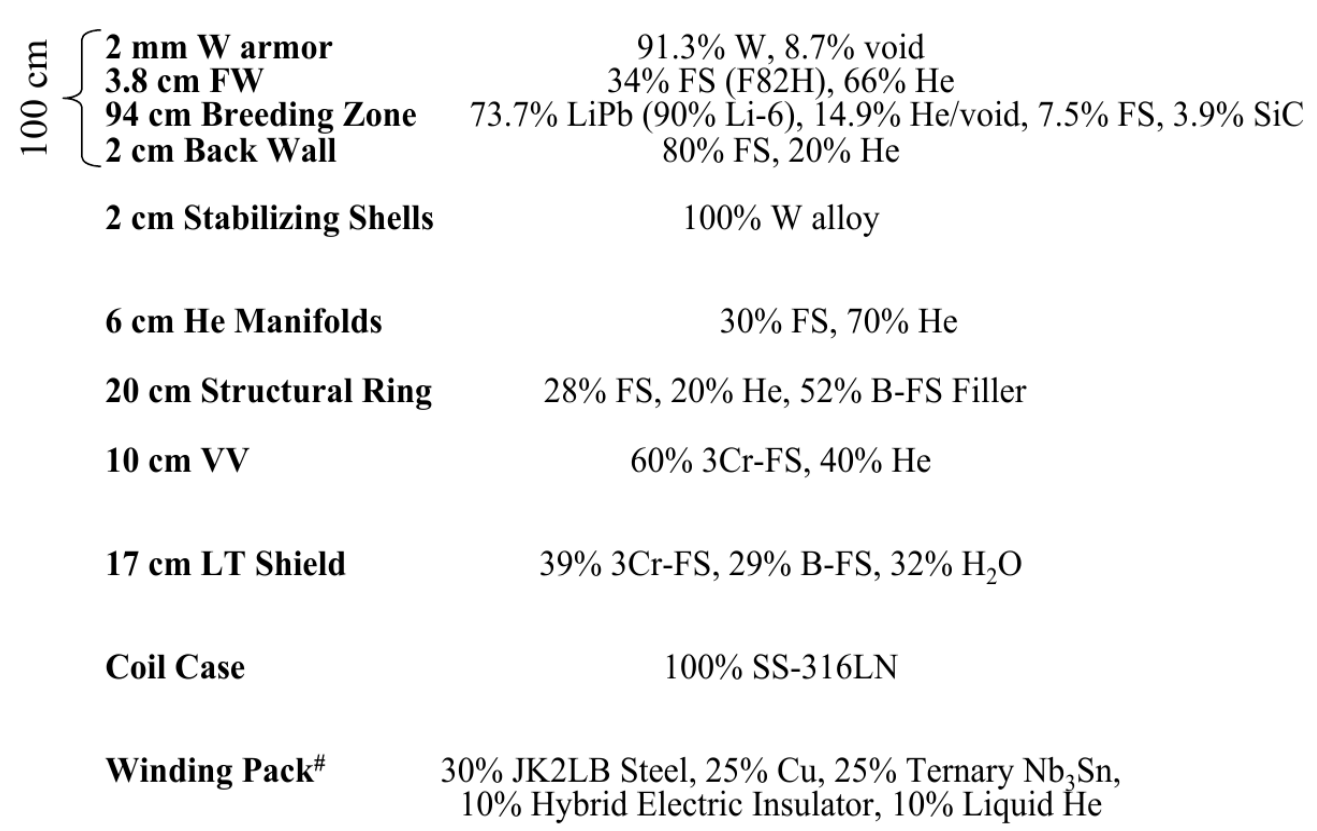
\includegraphics[scale=0.2]{../plots/OB_comp.png}
  \label{fig:OB_comp}
\end{figure}
\begin{figure}[h!]
  \centering
  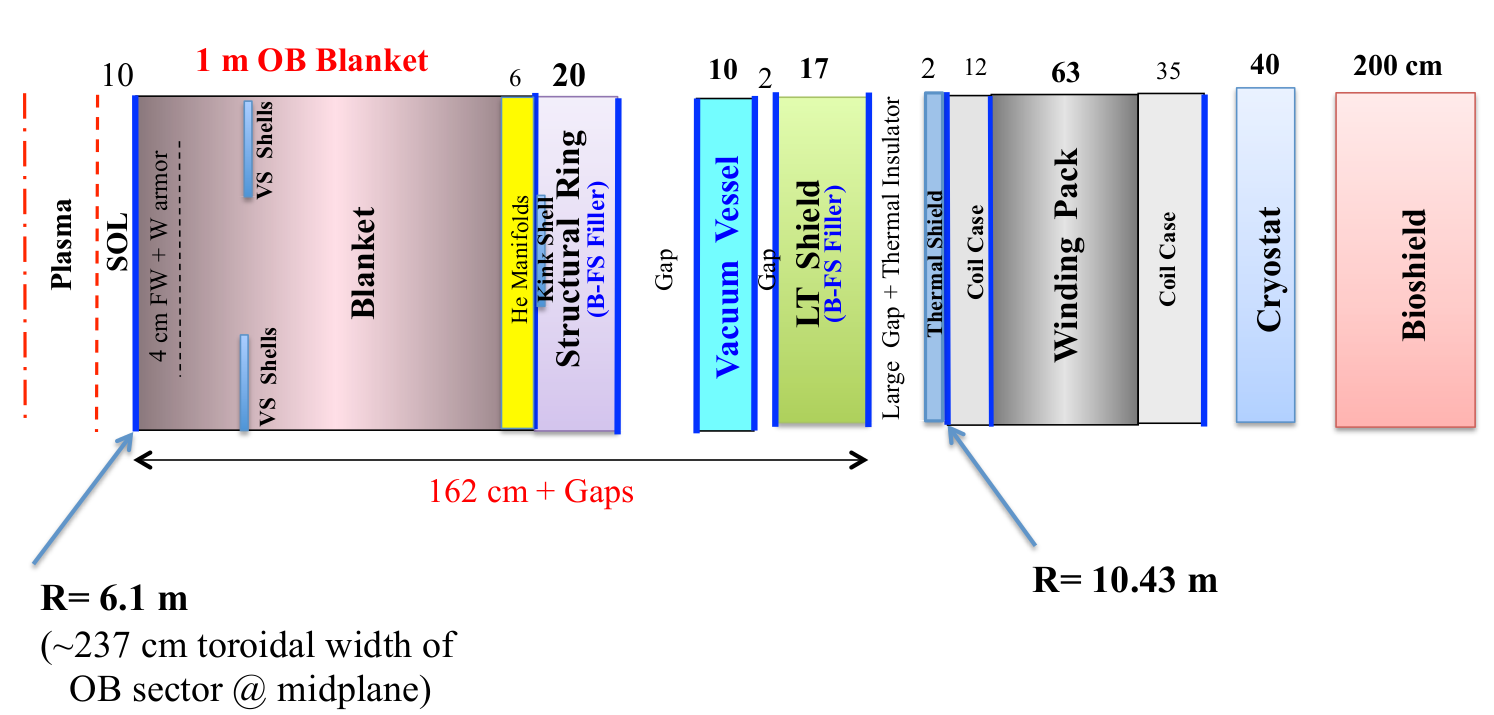
\includegraphics[scale=0.2]{../plots/OB_radial.png}
  \caption{The OB radial build}
  \label{fig:OB_radial}
\end{figure}

\subsection{Full 3D Build} \label{Full 3D Build}
The shielding and blanket optimization described in subsection (\ref{Configuration}) resulted in a full definition of the major materials and dimensions that were used to produce the 3D assembly CAD model. Shown in Figure \ref{fig:Full3D} is a cross section of one sector with the major regions identified on the figure. The model consists of 16 IB and OB sectors with \SI{2}{cm}assembly gaps. The facility has a major radius of \SI{4.8}{m} and a minor radius of \SI{1.2}{m}.
\begin{figure}[h!]
  \centering
  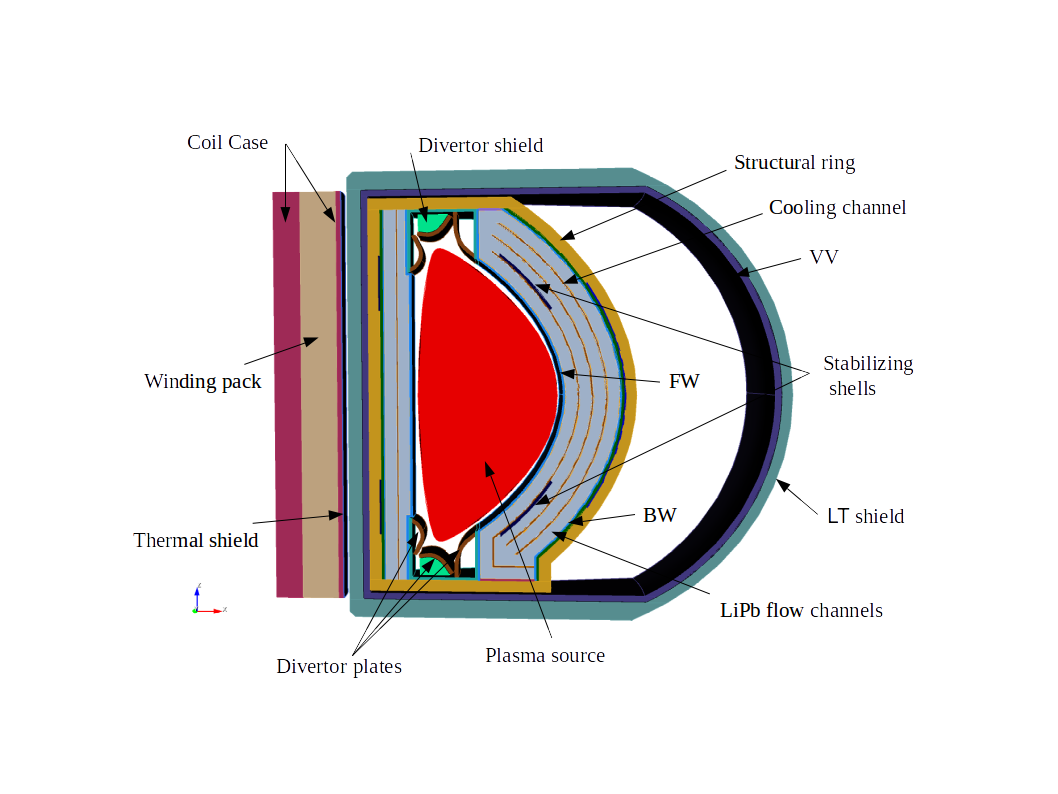
\includegraphics[scale=0.35]{../plots/full_3d.png}
  \caption{The full 3D CAD model of a single FESS-FNSF sector}
  \label{fig:Full3D}
\end{figure}

\section{Analysis Tools} \label{Analysis Tools}
As will be discussed in section (\ref{Tritium Breeding Calculations}), calculation of the TBR with high fidelity has to be achieved in order to confirm the adequacy of the configuration of the facility for tritium self-sufficiency. Based on previous analyses with similar models, some margins are considered in the design phase such that the final integration of all engineering systems in the facility will ensure a TBR $>$ 1. One of the margins \cite{ref_4} considered in the design phase of the facility is directly related to deficiencies in modeling resulting from approximations introduced to facilitate the analysis especially the neutron/photon transport calculations. In this study the approximations were applied to design details which are known – based on accumulated experience with previous models - to be of less importance regarding neutron/photon transport calculations besides slowing down the simulations if included. Such design details include; the detailed structure of the first wall “FW” and its He cooling system, the internal structure of the blanket cooling channels, and the internal structure of the He manifolds. Those regions are known to show little/no difference if modeled in detail or homogenized with a proper assignment of volume averaged material compositions.\vspace{5mm}

State-of-the-art analysis tools were utilized in this study which enabled working with the full 3-D model with all the internal details defined in the CAD, such as blanket internals and side/back/front walls, which are known to play a key role in TBR degradation. This work was performed with DAG-MCNP5, a version of MCNP5 \cite{ref_5} that has been enhanced by the DAGMC \cite{ref_6} toolkit. Coupled with MCNP5, DAGMC provides remarkable capabilities for the analysis of complex fusion facilities by utilizing acceleration techniques to achieve efficient ray tracing directly on CAD solid models without the need to translate the geometry/model to the native input representation of the transport code. Other software tools were used for mesh representation of the geometry and application of transport variance reduction techniques for deep penetration in regions behind the shields and the fusion evaluated nuclear data library (FENDL2.1)\cite{ref_7} was used in this analysis. Utilization of such sophisticated tools allowed reducing the approximations involved in the analysis by incorporating fine details which previously represented a challenge.\vspace{5mm}

The Shutdown dose rate (SDDR) analysis of the facility also plays a key role in the design phase. In the current study the r2s \cite{ref_8} workflow was used to perform the activation and shutdown dose rate calculations in one sector (without any penetrations or ports) of the facility with a simplified irradiation scenario. The analysis involved performing neutron transport calculations followed by nuclear inventory analysis using ALARA \cite{ref_9} code and then finally a photon transport calculation step using the produced decay gamma sources distribution for sampling.    

\subsection{Neutron Source Modeling} \label{Neutron Source Modelling}
An MCNP sampling routine was written to sample the neutrons for the transport calculations compared to the previous workflow which utilized either a simplified 3-region or R-Z sources. The physical parameters defining the plasma source \cite{ref_3} are: fusion power = \SI{518}{MW}, major radius = \SI{4.8}{m}, minor radius = \SI{1.2}{m}, elongation = 2.2, triangularity = 0.625, Shafranov shift = \SI{0.144}{m}, ion density in the pedistal, seperatrix, and core regions = 1x10\textsuperscript{20}/m\textsuperscript{3}, 0.56x10\textsuperscript{20}/m\textsuperscript{3}, and 1.6x10\textsuperscript{20}/m\textsuperscript{3} respectively with a peaking factor of 1.52 (peak to volume average), ion temperature in the pedistal, seperatrix, and core regions  = \SI{4}{keV}, \SI{100}{eV}, and \SI{22}{keV} respectively with a peaking factor of 2.25 (peak to volume average), and pedistal radius = \SI{1.14}{m}.
\begin{figure}[h!]
  \centering
  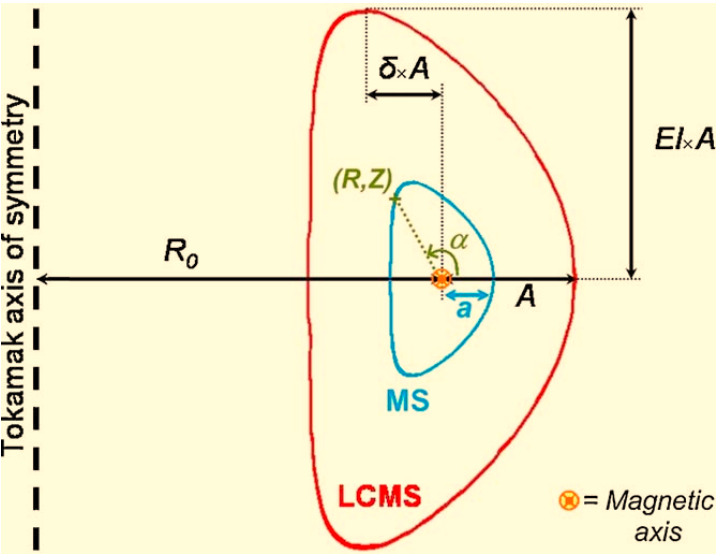
\includegraphics[scale=0.2]{../plots/Analytic_source.png}
  \caption{The analytic source configuration}
  \label{fig:Analytic_source}
\end{figure}

\section{Neutron Wall Loading} \label{Neutron Wall Loading}
The first step in the analysis applied to the full 3-D model involved calculations of the NWL distributions at the IB \& OB FWs, the inner \& outer divertor plates, and the middle divertor plate (dome). The vertical distribution of the NWL at the FWs (figure \ref{fig:NWL FWs}) and inner \& outer divertor plates (figure \ref{fig:NWL 2Divs}) were calculated over segments $\sim$ \SI{10}{cm} high. The radial distribution of the NWL at the dome is shown in figure \ref{fig:NWL Dome}. Table \ref{NWL peak and average values} shows the calculated peak and average values at the FWs and divertors. The peak values at the FWs occur at the midplane while for the inner and outer divertors it occurs at the bottom portion of the plate where it's closer to the plasma source. For the inner dome the peak value occurs in the middle.  
\begin{table}[h!]
	\caption{NWL peak and average values}
	\label{NWL peak and average values}
	\begin{tabular}{ |c|c|c|c| } 
		\hline
		 {} & Peak NWL [MW/m\textsuperscript{2}] & Average NWL [MW/m\textsuperscript{2}] \\
		\hline
		{OB FW} & 1.75 $\pm$ 0.11\% & 1.35 \\
		\hline
		{IB FW} & 1.31 $\pm$ 0.17\% & 0.86 \\
		\hline
		{Inner Divertor} & 0.79 $\pm$ 0.25\% & 0.32 \\
		\hline
		{Dome} & 0.66 $\pm$ 0.27\% & 0.49 \\
		\hline
		{Outer Divertor} & 0.76 $\pm$ 0.14\% & 0.35 \\
		\hline
		{3 Divertor plates} & 0.79 $\pm$ 0.13\% & 0.38 \\
		\hline
	\end{tabular}
\end{table}
 \begin{figure}[h!]
  \centering
  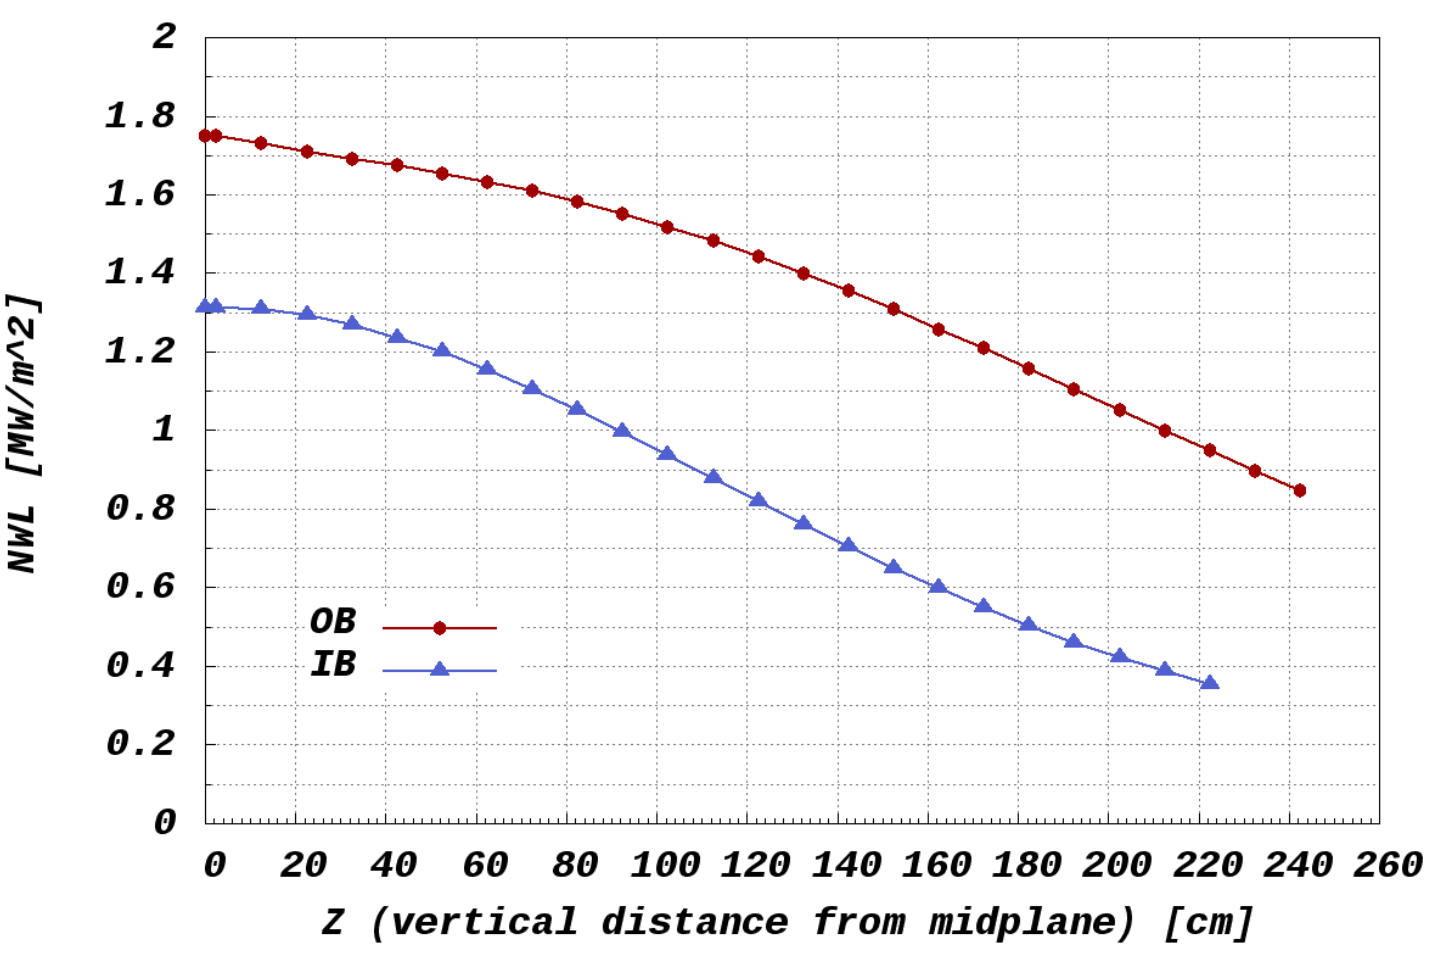
\includegraphics[scale=0.2]{../plots/NWL_FWs.png}
  \caption{The NWL vertical distribution at IB $\&$ OB FW}
  \label{fig:NWL FWs}
\end{figure}
\begin{figure}[h!]
  \centering
  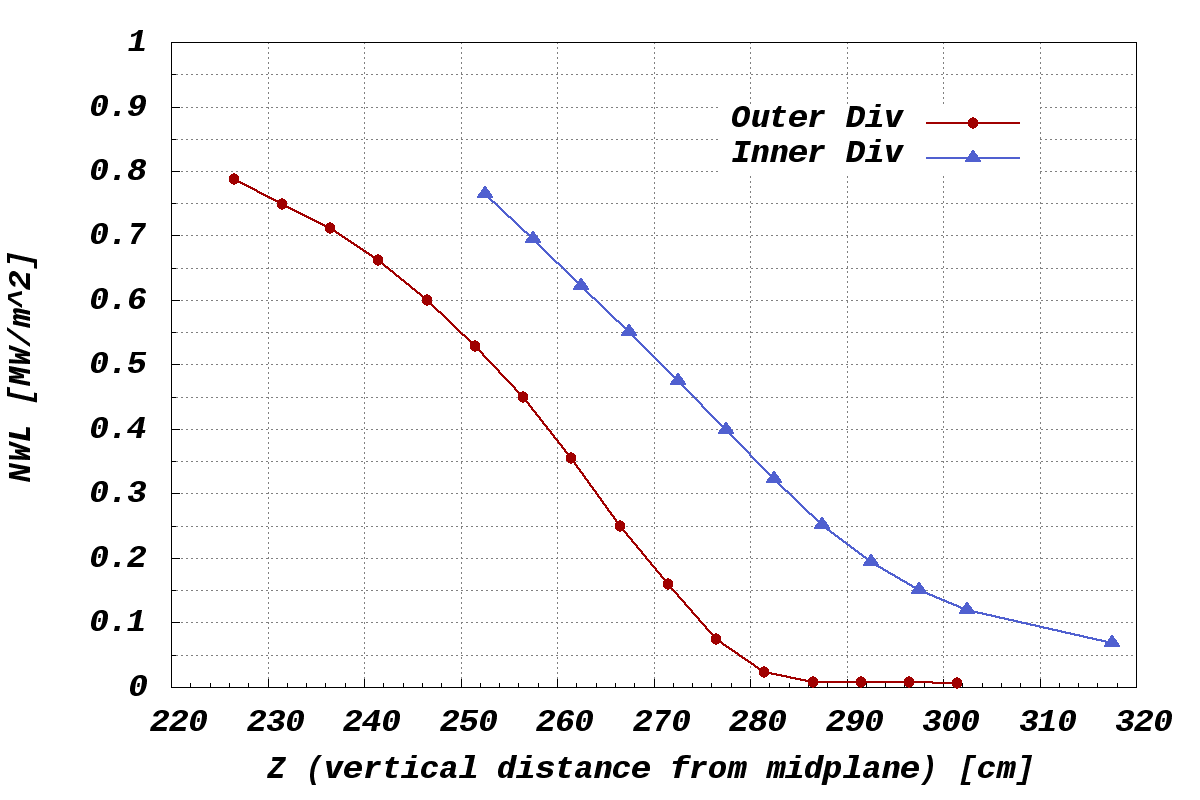
\includegraphics[scale=0.3]{../plots/NWL_2divs.png}
  \caption{The NWL vertical distribution at the inner and outer divertors}
  \label{fig:NWL 2Divs}
\end{figure}
\begin{figure}[h!]
	\centering
	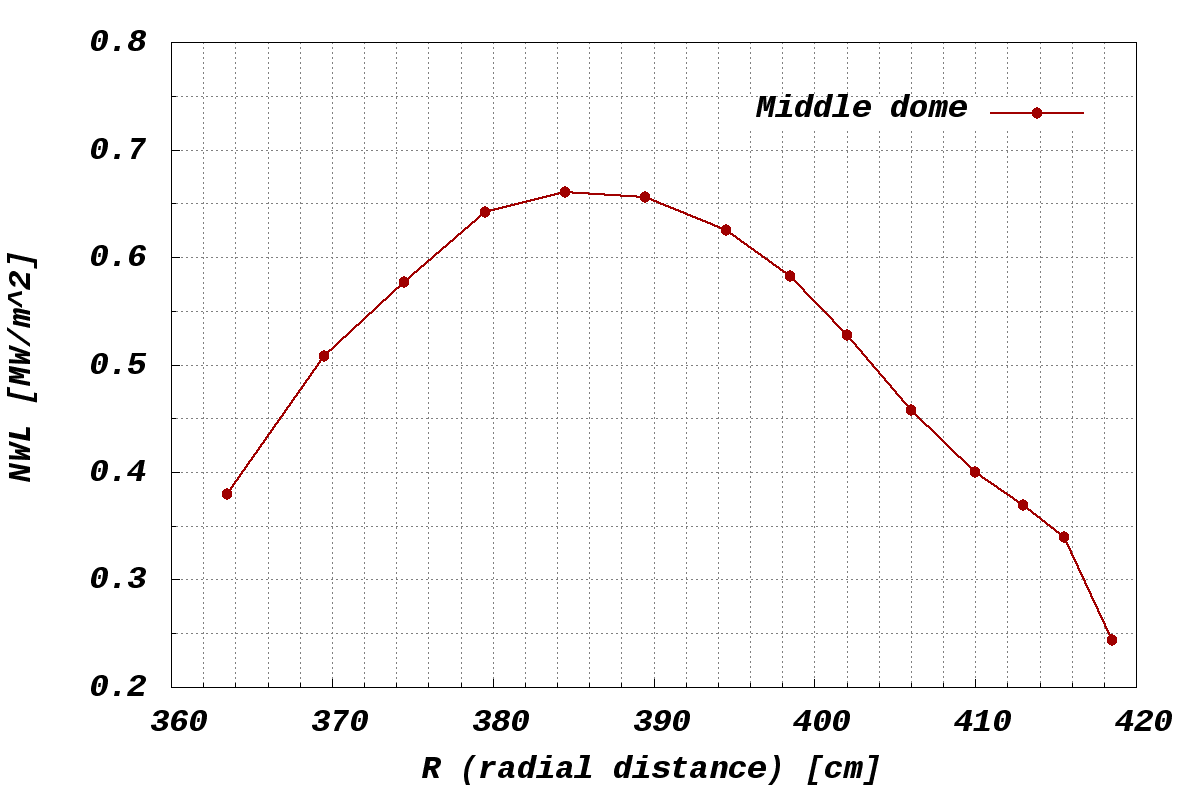
\includegraphics[scale=0.3]{../plots/NWL_div.png}
	\caption{The NWL distribution at the dome}
	\label{fig:NWL Dome}
\end{figure}

\section{Tritium Breeding Calculations} \label{Tritium Breeding Calculations}
The rich fusion research literature shows a growing interest to achieve ignition via the D-T fuel cycle and due to the scarcity of T in nature and the high cost of T consumed by fusion power plants (55.6 kg/full power year (FPY)/GW) \cite{ref_4}, all power plants developed to date that employs the D-T fuel cycle are required to breed T in blankets surrounding the plasma. As a result the need for TBR (ratio of tritium bred in the blankets to that consumed in the plasma) calculations with high certainty grew substantially and the TBR is considered an essential metric in the design phase.\vspace{5mm}

The blanket of choice for the FESS-FNSF project is the dual cooled lead-lithium (DCLL) \cite{ref_11} blanket. The blanket consists of $\pm$ \SI{20}{cm} radial/toroidal flow channels of LiPb eutectic (15.7 at\% Li (90\% Li6 enrichment) and 84.3 at\% Pb) surrounded by \SI{0.5}{cm} SiC FCI (flow channel insert) and \SI{0.2}{cm} layer of LiPb. The blanket is cooled by helium at high pressure (\SI{8}{MPa}) which is also used for heat removal in other components such as FW and blanket side/back/front walls. The blanket also serves other purposes besides breeding T such as the removal of volumetric heat deposited by fast neutrons from the plasma and shielding the outer components such as the structural ring (SR), the vacuum vessel (VV), and the magnets.

\subsection{TBR Workflow} \label{TBR Workflow}
A workflow for the calculation of the TBR of the facility was developed which involved assessing the impact of individual design elements/details on the breeding capacity. The workflow consists mainly of a multistep approach to calculate the TBR by starting the analysis with a CAD model with a simplified breeding blanket and at each step a new detail is added such as the He flow channels, the side walls, etc. and the resulting TBR of the facility is calculated. The TBR results are shown in figure \ref{fig:TBR chart}. \vspace{5mm}

Step 1 is a reference case showing the TBR for an infinite cylinder of LiPb surrounded by shields and utilised a coaxial plasma source. In step 2, the model was constructed of 16 sectors each consisting of IB and OB breeding blankets surrounded by shields and divertors with \SI{2}{cm} assembly gaps between the sectors. The 3-D configuration with such a limited radial thickness and poloidal coverage resulted in a TBR drop of 19.74\%. The assignment of the homogenized composition (34\% ferritic steel (FS), 66\% He) to the \SI{3.8}{cm} thick IB and OB FWs (step 3) resulted in a TBR drop of 8.7\%. Modeling of side walls (same thickness and composition as FW) and the \SI{2}{cm} thick back walls (80\% FS, 20\% He) (step 4) resulted in an additional TBR drop of 2.79\%. Defining the main LiPb flow channels by modeling the \SI{1.5}{cm} cooling channels with an assigned composition (58\% FS, 42\% He) (step 5) resulted in a further drop of 3.95\%. Assigning 34\% SiC to the \SI{0.5}{cm} FCI (step 6) resulted in a drop of 4.6\%. Adding the \SI{2}{cm} IB and OB stabilizing shells (W alloy) (step 7) resulted in a drop of 4.11\%.
\begin{figure}[h!]
  \centering
  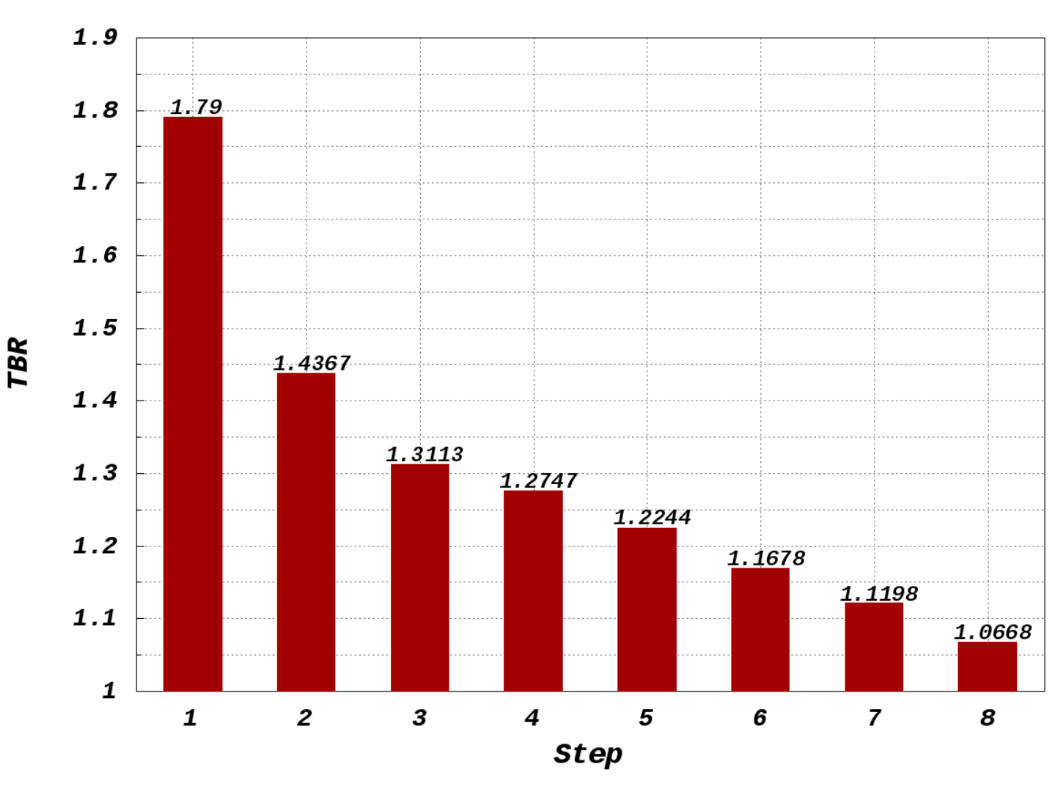
\includegraphics[scale=0.3]{../plots/TBR_chart.png}
  \caption{TBR chart}
  \label{fig:TBR chart}
\end{figure}

\subsection{Penetrations and Ports} \label{Penetrations and Ports}
The facility has 12 mid-plane and 6 off-mid-plane ports, the effect of which was assessed by adding each type of ports to the respective sectors and calculate the facility overall TBR and the corresponding drop (compared to step 7). It's worth noting that the ports were modeled in detail; frames, gaps, blanket frames, and internal structures were included in the CAD model. Adding the material testing module (MTM) (in 1 sector, \SI{1}{m\textsuperscript{2}} at FW) resulted in a drop of 0.313\%. The facility has 4 tritium breeding modules (TBM) (in 4 sectors, \SI{1}{m\textsuperscript{2}} each at FW), for purposes of testing different breeding concepts, resulting in a drop in the TBR of 0.2\%. The three plasma diagnostics ports resulted in a drop of 0.95\%. Including two neutral beam injectors (NBI) (in 4 sectors, \SI{1.9}{m\textsuperscript{2}} each at FW) reduced the TBR by 1.63\%. \vspace{5mm}

The remaining ports; IC (in 1 sector, \SI{2}{m\textsuperscript{2}} at FW), LH (in 1 sector, \SI{1.5}{m\textsuperscript{2}} at FW), EC (in 1 sector, \SI{0.675}{m\textsuperscript{2}} at FW), Fueling (in 1 sector, \SI{0.04}{m\textsuperscript{2}} at FW), Disruption mitigation (in 1 sector, \SI{0.04}{m\textsuperscript{2}} at FW), and two Divertor diagnostics (in 1 sector, \SI{0.15}{m\textsuperscript{2}} each at FW) resulted in a TBR drop of 0.71\%, 0.5\%, 0.23\%, 0.02\%, 0.02\%, and 0.08\%, respectively. A final step (step 8 on figure 3) with all penetrations included at the same time resulted in a drop of 4.95\%. A planar cross section of the facility with all penetrations identified is shown in figure \ref{fig:Ports}.
\begin{figure}[h!]
  \centering
  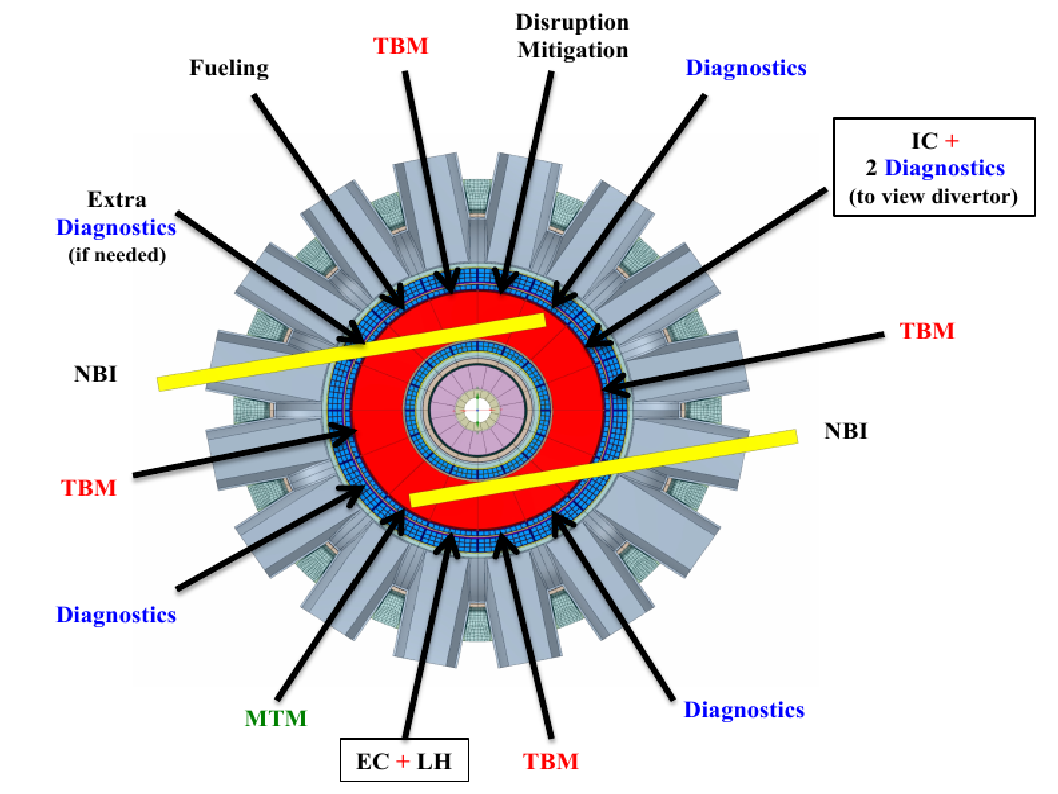
\includegraphics[scale=0.3]{../plots/ports.png}
  \caption{TBR chart}
  \label{fig:Ports}
\end{figure}

\subsection{Li-6 Enrichment} \label{Li-6 Enrichment}
One of the advantages of the DCLL blanket is allowing the control of the T bred by controlling the  Li6 enrichment in LiPb in the main flow channels. Controlling Li6 enrichment is necessary to avoid dealing with a surplus or shortage of T. Analyses were performed to test the effect of changing Li6 enrichment on the overall TBR of the facility (with all penetrations and ports included) and it was found that the TBR dropped to $1.0191\pm 0.03\%$, $0.9892\pm 0.03\%$, and $0.9513\pm 0.03\%$ for 70\%, 60\%, and 50\% Li6  enrichment, respectively. The TBR satisfies the tritium breeding requirement of 1.04 with ~ 80\% Li6 enrichment and the results are shown in figure 6.
\begin{figure}[h!]
  \centering
  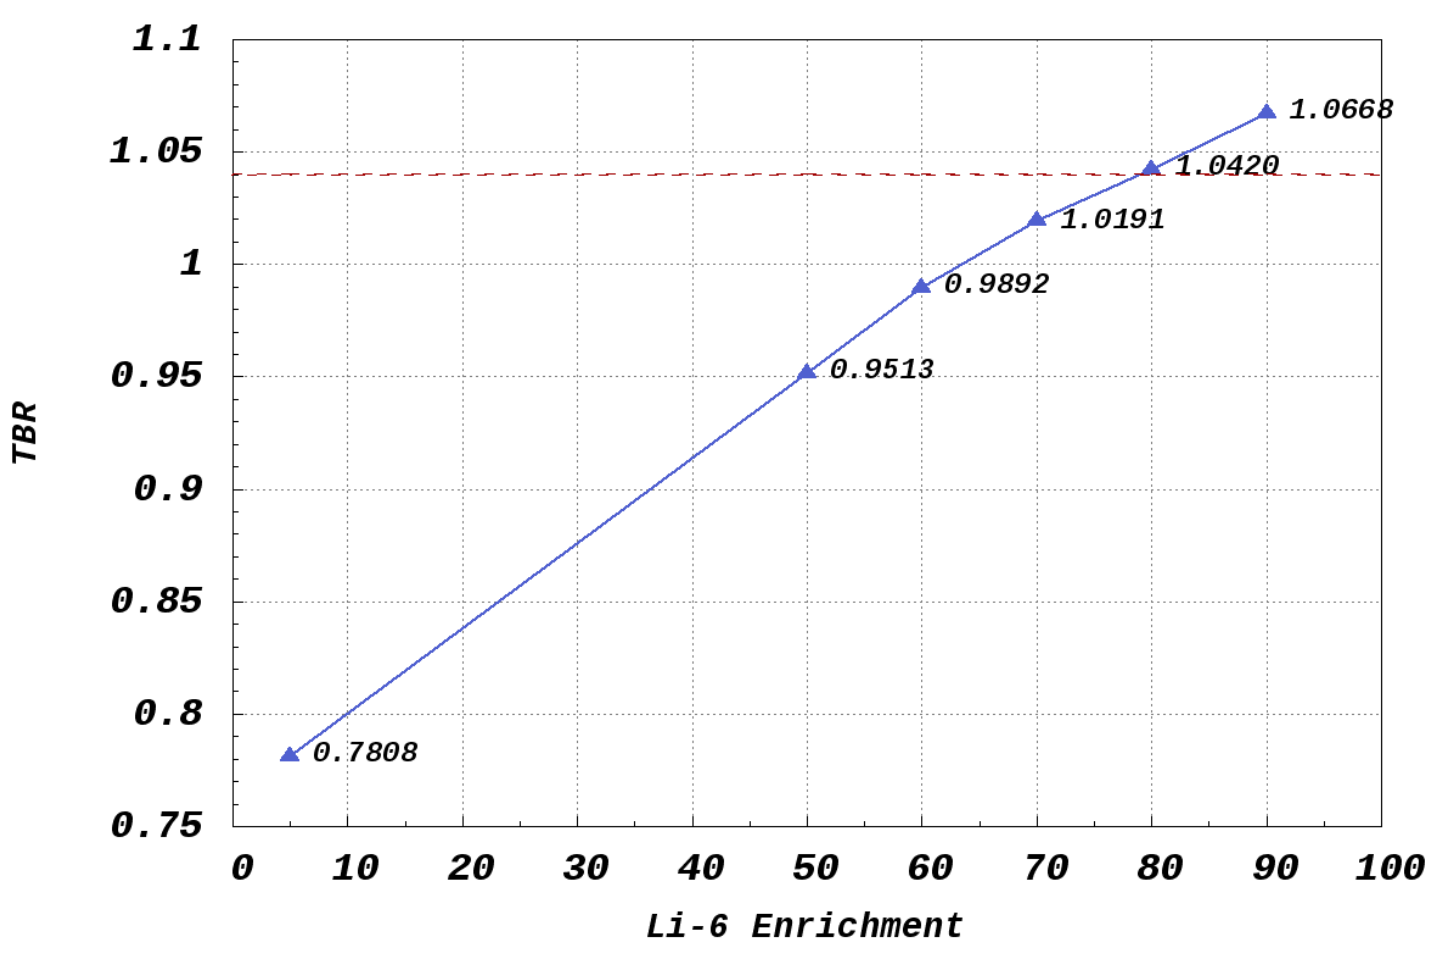
\includegraphics[scale=0.2]{../plots/Li6_enrichment.png}
  \caption{The facility overall TBR vs Li6 enrichment}
  \label{fig:Li6_enrichment}
\end{figure}

\subsection{TBR mapping} \label{TBR mapping}
One of the design concepts implemented in the current design – based on experience with previous models – is keeping the mid-plane clear of any ports/penetrations as practically achievable. The current model has a peak NWL of 1.75 and \SI{1.31}{MW/m\textsuperscript{2}} at the OB and IB mid-planes, respectively. This could directly be related to the calculated TBR showing that more T is produced near the mid-plane compared to the upper and lower (poloidal direction) or back (radial direction) of both the \SI{0.5}{m} IB and the \SI{1}{m} OB blankets.\vspace{5mm}

Using DAG-MCNP5 mesh tally capabilities the T production was mapped in the IB and OB blankets of one sector as shown in figure \ref{fig:step7} for step 7 and figure \ref{fig:NBI} for the NBI. Figure \ref{fig:step7} also shows a reduction in TBR behind the stabilizing shells due to the absorption of neutrons by W. Including any penetrations in the mid-plane will have an effect on the overall TBR by reducing the active volume of the blanket where it's most effective for T breeding, even though there may be slightly enhanced local T breeding far inside the blanket due to streaming of neutrons.
\begin{figure}[h!]
  \centering
  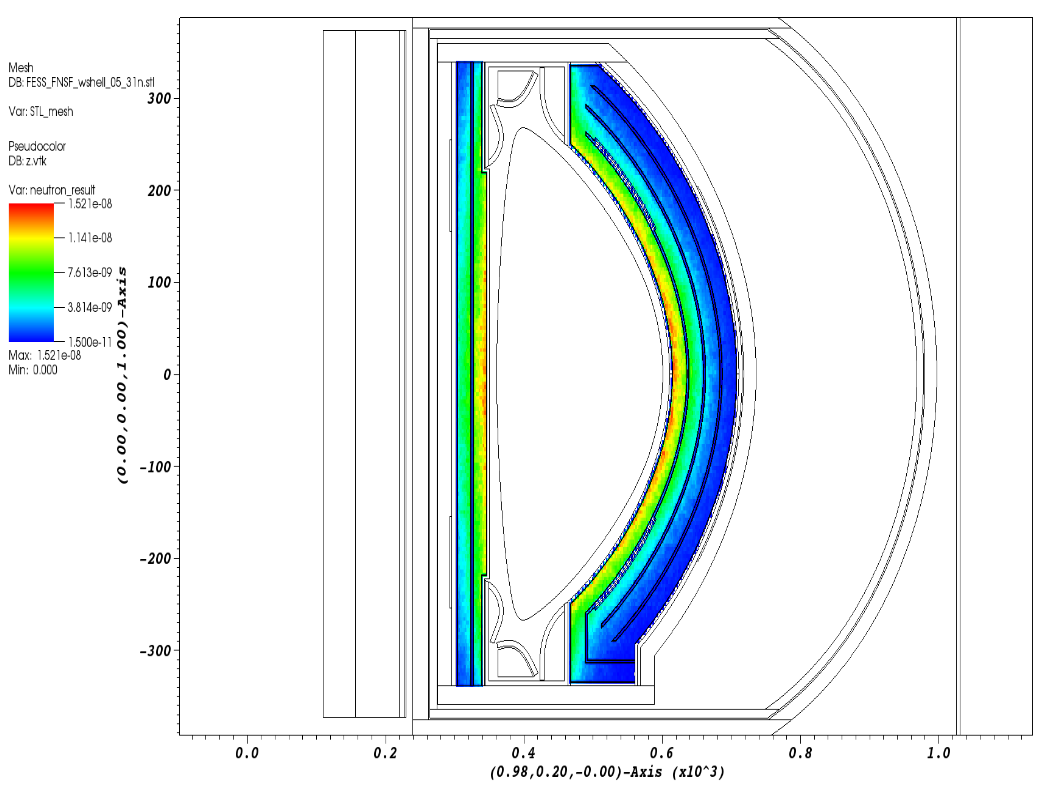
\includegraphics[scale=0.4]{../plots/step7.png}
  \caption{The tritium production mapping in one sector (without ports)}
  \label{fig:step7}
\end{figure}
\begin{figure}[h!]
  \centering
  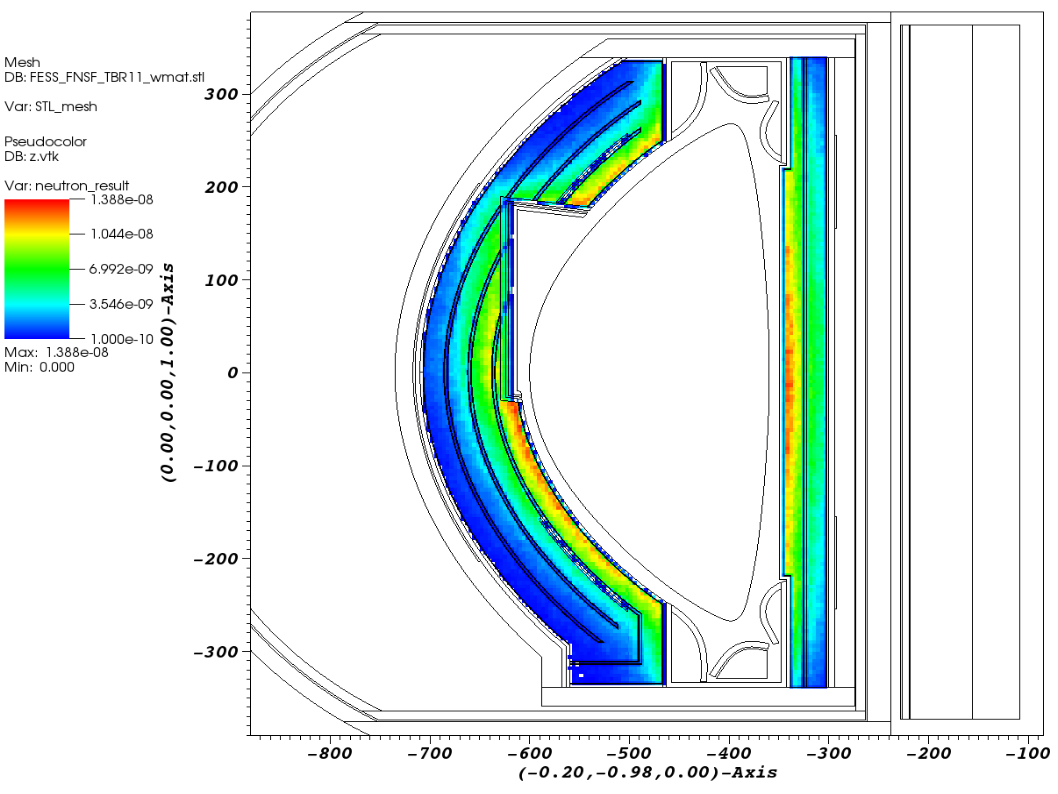
\includegraphics[scale=0.4]{../plots/NBI.png}
  \caption{The tritium production mapping in one sector (with NBI)}
  \label{fig:NBI}
\end{figure}

\section{Radiation Damage} \label{Radiation Damage}
The shielding analysis follows the tritium breeding blanket optimization to provide the needed protection of the lifetime components. The main shielding design philosophy (as employed in previous designs \cite{ref_10}) is that every layer provides protection to the following layers such that collectively they would protect the out-of-vessel components such as the magnets. For example, in addition to the T breeding, the blanket (both the IB and OB) is supposed to provide protection for the structural ring and in turn both would protect the vacuum vessel and finally all three layers would attenuate the neutron and gamma fluxes to such low levels to protect the magnets.

\subsection{dpa, He/H production} \label{dpa, He/H production}
The damage caused by irradiation to the in-vessel components is an important factor in the selection of materials in the design phase. The radiation damage can be quantified using two main parameters; displacement per atom (dpa) and gas (H and He) production. These parameters impact the lifetime of structural components and the potential for reweldability after irradiation.\vspace{5mm}

For the FW, the peak values calculated at the mid-plane are shown in table \ref{Radiation damage values for the FW and VV}. The radial distribution of the damage to the ferretic steel alloy (F82H) is shown in figure \ref{fig:Radial Damage}. It's worth noting that there is a slight increase in the He and H production near the end of the blanket at \SI{700}{cm} due to the strong neutron reflection from the SR/VV/shield. The reweldability of the VV is directly related to the levels of H and He produced during the operation and that leads to setting a limit of \SI{1}{He appm} which shouldn't be exceeded at any time during plant operation. An issue that needs to be addressed is the streaming through the assembly gaps (\SI{2}{cm} between the OB and IB sectors) and all penetrations described in section \ref{Penetrations and Ports} which will cause peaking in radiation damage to the exposed portions of the VV. The results of the damage at the VV mid-plane (away from the NBIs) are listed in table \ref{Radiation damage values for the FW and VV}.   
\begin{table}
	\caption{Radiation damage values for the FW and VV}
	\label{Radiation damage values for the FW and VV}
	\begin{tabular}{ |c|c|c|c|c| } 
		\hline
		{} & \multicolumn{2}{|c|}{FW} & \multicolumn{2}{|c|}{VV} \\
		\hline
		{} & IB & OB & IB & OB \\
		\hline
		\multirow{2}{6em}{Damage [dpa/FPY]} & 13.70 $\pm$ 1.53\% & 15.25 $\pm$ 0.92\% & 0.1495 $\pm$ 0.64\% & 0.0114 $\pm$ 0.36\%  \\
		& {} & {} & {} & {} \\
		\hline
		\multirow{2}{6em}{He [appm/FPY]} & 137.30 $\pm$ 2.52\% & 154.58 $\pm$ 1.41\% & 0.3109 $\pm$ 8.83\% & 0.0029 $\pm$ 13.81\%  \\
		& {} & {} & {} & {} \\
		\hline
		\multirow{2}{6em}{He/dpa ratio} & 10.02 & 10.14 & 2.08 & 0.26  \\
		& {} & {} & {} & {} \\
		\hline
		\multirow{2}{6em}{H [appm/FPY]} & 613.50 $\pm$ 2.42\% & 691.94 $\pm$ 1.35\% & 0.2462 $\pm$ 8.92\% & 0.0025 $\pm$ 12.99\%  \\
		& {} & {} & {} & {} \\
		\hline
	\end{tabular}
\end{table}
\begin{figure}[h!]
  \centering
  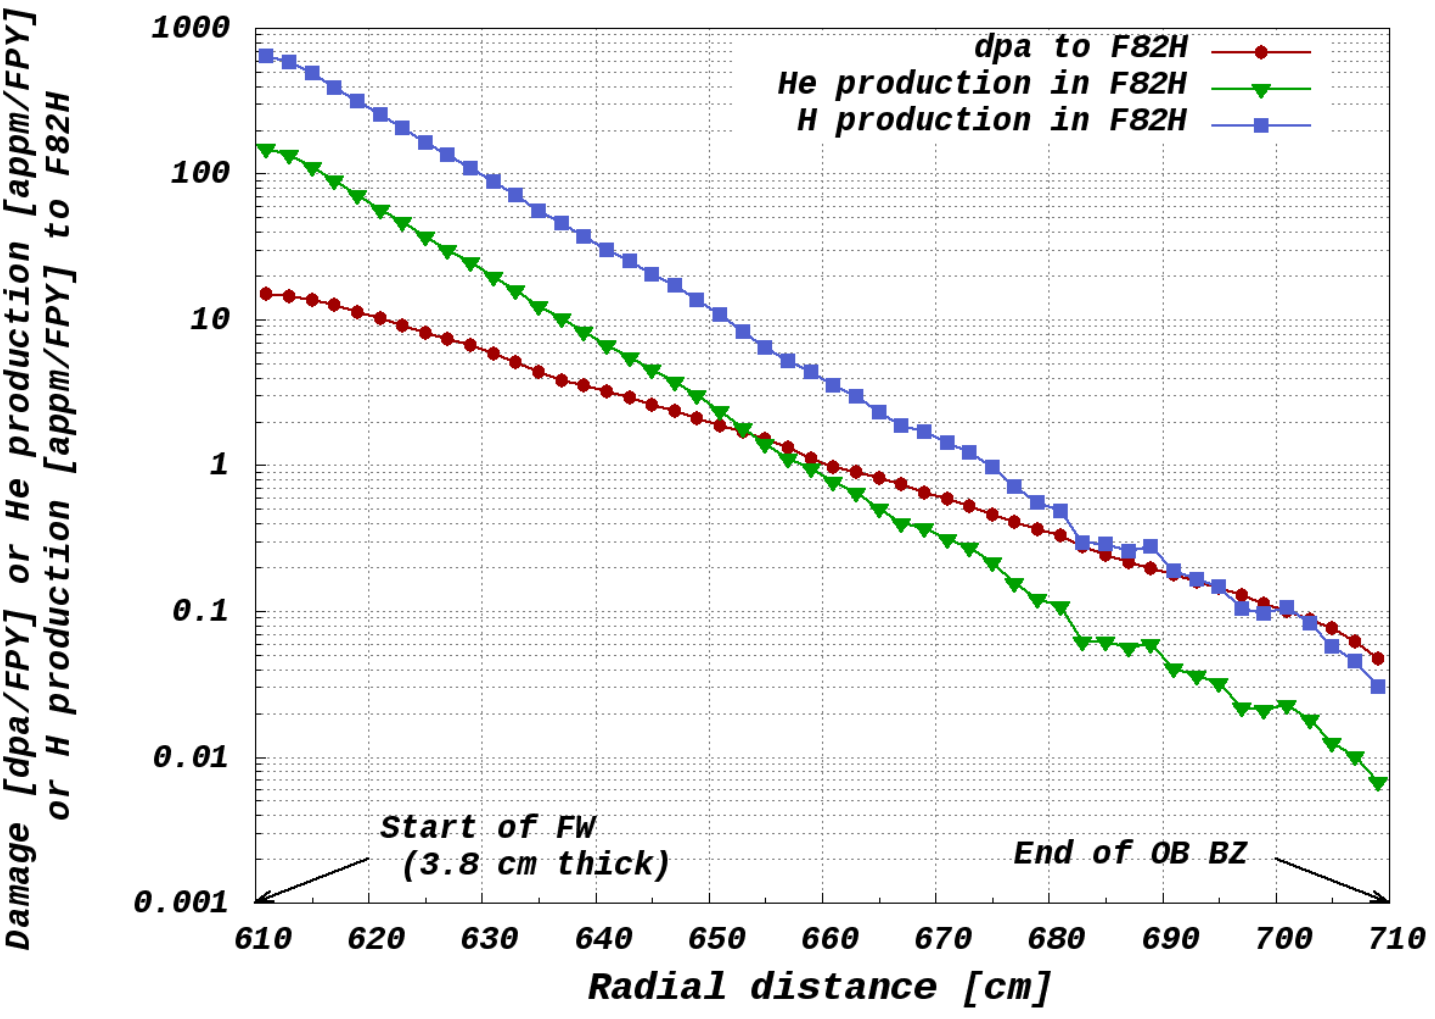
\includegraphics[scale=0.2]{../plots/radialdamage.png}
  \caption{The radial distribution of radiation damage at OB}
  \label{fig:Radial Damage}
\end{figure}

\subsection{Magnet damage} \label{Magnet damage}
\providecommand{\e}[1]{\ensuremath{\times 10^{#1}}}
The magnet is a critical component of the facility and is considered the main focus of all shielding optimization efforts. Following the shield design philosophy stated previously, the 3-D neutronics analysis confirmed that the radiation levels at the magnet winding pack (WP) met the limits set by the magnet designers. Calculations showed that the fast (E $>$ \SI{0.1}{MeV}) neutron fluence at the WP 1.35\e{18} $\pm$ 4.58\% n/cm\textsuperscript{2} is well below the limit (5\e{18} n/cm\textsuperscript{2}). The LT shield behind the VV has WC (37\%) and H2O (33\%) which combined have superior shielding capacity in attenuating the neutron flux. The peak nuclear heating at the coil case “CC” is 0.26 $\pm$ 2.55\% mW/cm\textsuperscript{3}, below the limit of \SI{2}{mW/cm\textsuperscript{3}}. The peak dpa to the Cu stabilizer is 9.54\e{-5} $\pm$ 4.1\% dpa/FPY, also below the limit of 10\e{-4} dpa/FPY.

\section{Shutdown Dose Rate Calculations} \label{Shutdown Dose Rate Calculations}
introduction and r2s worflow
\subsection{SDR} \label{SDR}
\subsection{Decay Heat} \label{Decay Heat}

\section{Conclusions} \label{conclusion}

\newpage
\section{References}
\begin{thebibliography}{10} 
\bibitem{ref_1} 
C. E. KESSEL, et al., {“The Fusion Nuclear Science Facility, the Critical Step in the Pathway to Fusion Energy,” Fusion Science and Technology, vol. 68, p. 225–236 (2015).}
\bibitem{ref_2} 
L. El-Guebaly, et al., {“Design Approach for FESS-FNSF In-Vessel Components and Constraints Imposed on Radial/Vertical Build Definition,” presented at 22nd ANS Topical Meeting on the Technology of Fusion Energy (TOFE), August 22 -25, 2016, Philadelphia, PA. To be published in Fusion Science and Technology.}
\bibitem{ref_3}
Clement Fausser, et al., {“Tokamak D-T Neutron Source Models for Different Plasma Physics Confinement Modes.” Fusion Engineering and Design, vol. 87, p. 787–792 (2012).} 
\bibitem{ref_4}
L. A. EL-GUEBALY, et al., {“Toward the Ultimate Goal of Tritium Self-Sufficiency: Technical Issues and Requirements Imposed on ARIES Advanced Power Plants,” Fusion Engineering and Design, vol. 84, p. 2072-2083 (2009).}
\bibitem{ref_5}
X-5 Monte Carlo Team, {MCNP a General Monte Carlo N-Particle Transport Code Version 5, Tech. Rep. LA-CP-03-0245, Los Alamos National Laboratory, MCNP 5, (March 2005).}
\bibitem{ref_6}
{DAGMC: http://svalinn.github.io/DAGMC/}
\bibitem{ref_7}
D. L. ALDAMA and et al., {“FENDL2.1, Update of an Evaluated Nuclear Data Library for Fusion applications.” IAEA report INDC (NDS) 467, Vienna, Austria (2004).}
\bibitem{ref_8}
Y. Chen and U. Fischer, {"Rigorous MCNP based shutdown dose rate calculations: computational scheme, verification calculations and application to ITER." Fusion Engineering and Design, 63-64, 107–114 (2002).}
\bibitem{ref_9}
{https://github.com/svalinn/ALARA}
\bibitem{ref_10}
S. MALANG et al., {“Development of the Lead Lithium (DCLL) Blanket Concept,” Fusion Science and Technology, 60, 249 (2011).}
\bibitem{ref_11}
L. EL-GUEBALY and the ARIES Team, {“Overview of ARIES-RS Neutronics and Radiation Shielding: Key Issues and Main Conclusions,” Fusion Engineering and Design, vol. 38, p. 139 – 158 (1997).}
\end{thebibliography}

\end{document}